
% Default to the notebook output style

    


% Inherit from the specified cell style.




    
\documentclass[11pt]{article}

    
    
    \usepackage[T1]{fontenc}
    % Nicer default font (+ math font) than Computer Modern for most use cases
    \usepackage{mathpazo}

    % Basic figure setup, for now with no caption control since it's done
    % automatically by Pandoc (which extracts ![](path) syntax from Markdown).
    \usepackage{graphicx}
    % We will generate all images so they have a width \maxwidth. This means
    % that they will get their normal width if they fit onto the page, but
    % are scaled down if they would overflow the margins.
    \makeatletter
    \def\maxwidth{\ifdim\Gin@nat@width>\linewidth\linewidth
    \else\Gin@nat@width\fi}
    \makeatother
    \let\Oldincludegraphics\includegraphics
    % Set max figure width to be 80% of text width, for now hardcoded.
    \renewcommand{\includegraphics}[1]{\Oldincludegraphics[width=.8\maxwidth]{#1}}
    % Ensure that by default, figures have no caption (until we provide a
    % proper Figure object with a Caption API and a way to capture that
    % in the conversion process - todo).
    \usepackage{caption}
    \DeclareCaptionLabelFormat{nolabel}{}
    \captionsetup{labelformat=nolabel}

    \usepackage{adjustbox} % Used to constrain images to a maximum size 
    \usepackage{xcolor} % Allow colors to be defined
    \usepackage{enumerate} % Needed for markdown enumerations to work
    \usepackage{geometry} % Used to adjust the document margins
    \usepackage{amsmath} % Equations
    \usepackage{amssymb} % Equations
    \usepackage{textcomp} % defines textquotesingle
    % Hack from http://tex.stackexchange.com/a/47451/13684:
    \AtBeginDocument{%
        \def\PYZsq{\textquotesingle}% Upright quotes in Pygmentized code
    }
    \usepackage{upquote} % Upright quotes for verbatim code
    \usepackage{eurosym} % defines \euro
    \usepackage[mathletters]{ucs} % Extended unicode (utf-8) support
    \usepackage[utf8x]{inputenc} % Allow utf-8 characters in the tex document
    \usepackage{fancyvrb} % verbatim replacement that allows latex
    \usepackage{grffile} % extends the file name processing of package graphics 
                         % to support a larger range 
    % The hyperref package gives us a pdf with properly built
    % internal navigation ('pdf bookmarks' for the table of contents,
    % internal cross-reference links, web links for URLs, etc.)
    \usepackage{hyperref}
    \usepackage{longtable} % longtable support required by pandoc >1.10
    \usepackage{booktabs}  % table support for pandoc > 1.12.2
    \usepackage[inline]{enumitem} % IRkernel/repr support (it uses the enumerate* environment)
    \usepackage[normalem]{ulem} % ulem is needed to support strikethroughs (\sout)
                                % normalem makes italics be italics, not underlines
    

    
    
    % Colors for the hyperref package
    \definecolor{urlcolor}{rgb}{0,.145,.698}
    \definecolor{linkcolor}{rgb}{.71,0.21,0.01}
    \definecolor{citecolor}{rgb}{.12,.54,.11}

    % ANSI colors
    \definecolor{ansi-black}{HTML}{3E424D}
    \definecolor{ansi-black-intense}{HTML}{282C36}
    \definecolor{ansi-red}{HTML}{E75C58}
    \definecolor{ansi-red-intense}{HTML}{B22B31}
    \definecolor{ansi-green}{HTML}{00A250}
    \definecolor{ansi-green-intense}{HTML}{007427}
    \definecolor{ansi-yellow}{HTML}{DDB62B}
    \definecolor{ansi-yellow-intense}{HTML}{B27D12}
    \definecolor{ansi-blue}{HTML}{208FFB}
    \definecolor{ansi-blue-intense}{HTML}{0065CA}
    \definecolor{ansi-magenta}{HTML}{D160C4}
    \definecolor{ansi-magenta-intense}{HTML}{A03196}
    \definecolor{ansi-cyan}{HTML}{60C6C8}
    \definecolor{ansi-cyan-intense}{HTML}{258F8F}
    \definecolor{ansi-white}{HTML}{C5C1B4}
    \definecolor{ansi-white-intense}{HTML}{A1A6B2}

    % commands and environments needed by pandoc snippets
    % extracted from the output of `pandoc -s`
    \providecommand{\tightlist}{%
      \setlength{\itemsep}{0pt}\setlength{\parskip}{0pt}}
    \DefineVerbatimEnvironment{Highlighting}{Verbatim}{commandchars=\\\{\}}
    % Add ',fontsize=\small' for more characters per line
    \newenvironment{Shaded}{}{}
    \newcommand{\KeywordTok}[1]{\textcolor[rgb]{0.00,0.44,0.13}{\textbf{{#1}}}}
    \newcommand{\DataTypeTok}[1]{\textcolor[rgb]{0.56,0.13,0.00}{{#1}}}
    \newcommand{\DecValTok}[1]{\textcolor[rgb]{0.25,0.63,0.44}{{#1}}}
    \newcommand{\BaseNTok}[1]{\textcolor[rgb]{0.25,0.63,0.44}{{#1}}}
    \newcommand{\FloatTok}[1]{\textcolor[rgb]{0.25,0.63,0.44}{{#1}}}
    \newcommand{\CharTok}[1]{\textcolor[rgb]{0.25,0.44,0.63}{{#1}}}
    \newcommand{\StringTok}[1]{\textcolor[rgb]{0.25,0.44,0.63}{{#1}}}
    \newcommand{\CommentTok}[1]{\textcolor[rgb]{0.38,0.63,0.69}{\textit{{#1}}}}
    \newcommand{\OtherTok}[1]{\textcolor[rgb]{0.00,0.44,0.13}{{#1}}}
    \newcommand{\AlertTok}[1]{\textcolor[rgb]{1.00,0.00,0.00}{\textbf{{#1}}}}
    \newcommand{\FunctionTok}[1]{\textcolor[rgb]{0.02,0.16,0.49}{{#1}}}
    \newcommand{\RegionMarkerTok}[1]{{#1}}
    \newcommand{\ErrorTok}[1]{\textcolor[rgb]{1.00,0.00,0.00}{\textbf{{#1}}}}
    \newcommand{\NormalTok}[1]{{#1}}
    
    % Additional commands for more recent versions of Pandoc
    \newcommand{\ConstantTok}[1]{\textcolor[rgb]{0.53,0.00,0.00}{{#1}}}
    \newcommand{\SpecialCharTok}[1]{\textcolor[rgb]{0.25,0.44,0.63}{{#1}}}
    \newcommand{\VerbatimStringTok}[1]{\textcolor[rgb]{0.25,0.44,0.63}{{#1}}}
    \newcommand{\SpecialStringTok}[1]{\textcolor[rgb]{0.73,0.40,0.53}{{#1}}}
    \newcommand{\ImportTok}[1]{{#1}}
    \newcommand{\DocumentationTok}[1]{\textcolor[rgb]{0.73,0.13,0.13}{\textit{{#1}}}}
    \newcommand{\AnnotationTok}[1]{\textcolor[rgb]{0.38,0.63,0.69}{\textbf{\textit{{#1}}}}}
    \newcommand{\CommentVarTok}[1]{\textcolor[rgb]{0.38,0.63,0.69}{\textbf{\textit{{#1}}}}}
    \newcommand{\VariableTok}[1]{\textcolor[rgb]{0.10,0.09,0.49}{{#1}}}
    \newcommand{\ControlFlowTok}[1]{\textcolor[rgb]{0.00,0.44,0.13}{\textbf{{#1}}}}
    \newcommand{\OperatorTok}[1]{\textcolor[rgb]{0.40,0.40,0.40}{{#1}}}
    \newcommand{\BuiltInTok}[1]{{#1}}
    \newcommand{\ExtensionTok}[1]{{#1}}
    \newcommand{\PreprocessorTok}[1]{\textcolor[rgb]{0.74,0.48,0.00}{{#1}}}
    \newcommand{\AttributeTok}[1]{\textcolor[rgb]{0.49,0.56,0.16}{{#1}}}
    \newcommand{\InformationTok}[1]{\textcolor[rgb]{0.38,0.63,0.69}{\textbf{\textit{{#1}}}}}
    \newcommand{\WarningTok}[1]{\textcolor[rgb]{0.38,0.63,0.69}{\textbf{\textit{{#1}}}}}
    
    
    % Define a nice break command that doesn't care if a line doesn't already
    % exist.
    \def\br{\hspace*{\fill} \\* }
    % Math Jax compatability definitions
    \def\gt{>}
    \def\lt{<}
    % Document parameters
    \title{Neural Modelling Synthesis}
    
    
    

    % Pygments definitions
    
\makeatletter
\def\PY@reset{\let\PY@it=\relax \let\PY@bf=\relax%
    \let\PY@ul=\relax \let\PY@tc=\relax%
    \let\PY@bc=\relax \let\PY@ff=\relax}
\def\PY@tok#1{\csname PY@tok@#1\endcsname}
\def\PY@toks#1+{\ifx\relax#1\empty\else%
    \PY@tok{#1}\expandafter\PY@toks\fi}
\def\PY@do#1{\PY@bc{\PY@tc{\PY@ul{%
    \PY@it{\PY@bf{\PY@ff{#1}}}}}}}
\def\PY#1#2{\PY@reset\PY@toks#1+\relax+\PY@do{#2}}

\expandafter\def\csname PY@tok@w\endcsname{\def\PY@tc##1{\textcolor[rgb]{0.73,0.73,0.73}{##1}}}
\expandafter\def\csname PY@tok@c\endcsname{\let\PY@it=\textit\def\PY@tc##1{\textcolor[rgb]{0.25,0.50,0.50}{##1}}}
\expandafter\def\csname PY@tok@cp\endcsname{\def\PY@tc##1{\textcolor[rgb]{0.74,0.48,0.00}{##1}}}
\expandafter\def\csname PY@tok@k\endcsname{\let\PY@bf=\textbf\def\PY@tc##1{\textcolor[rgb]{0.00,0.50,0.00}{##1}}}
\expandafter\def\csname PY@tok@kp\endcsname{\def\PY@tc##1{\textcolor[rgb]{0.00,0.50,0.00}{##1}}}
\expandafter\def\csname PY@tok@kt\endcsname{\def\PY@tc##1{\textcolor[rgb]{0.69,0.00,0.25}{##1}}}
\expandafter\def\csname PY@tok@o\endcsname{\def\PY@tc##1{\textcolor[rgb]{0.40,0.40,0.40}{##1}}}
\expandafter\def\csname PY@tok@ow\endcsname{\let\PY@bf=\textbf\def\PY@tc##1{\textcolor[rgb]{0.67,0.13,1.00}{##1}}}
\expandafter\def\csname PY@tok@nb\endcsname{\def\PY@tc##1{\textcolor[rgb]{0.00,0.50,0.00}{##1}}}
\expandafter\def\csname PY@tok@nf\endcsname{\def\PY@tc##1{\textcolor[rgb]{0.00,0.00,1.00}{##1}}}
\expandafter\def\csname PY@tok@nc\endcsname{\let\PY@bf=\textbf\def\PY@tc##1{\textcolor[rgb]{0.00,0.00,1.00}{##1}}}
\expandafter\def\csname PY@tok@nn\endcsname{\let\PY@bf=\textbf\def\PY@tc##1{\textcolor[rgb]{0.00,0.00,1.00}{##1}}}
\expandafter\def\csname PY@tok@ne\endcsname{\let\PY@bf=\textbf\def\PY@tc##1{\textcolor[rgb]{0.82,0.25,0.23}{##1}}}
\expandafter\def\csname PY@tok@nv\endcsname{\def\PY@tc##1{\textcolor[rgb]{0.10,0.09,0.49}{##1}}}
\expandafter\def\csname PY@tok@no\endcsname{\def\PY@tc##1{\textcolor[rgb]{0.53,0.00,0.00}{##1}}}
\expandafter\def\csname PY@tok@nl\endcsname{\def\PY@tc##1{\textcolor[rgb]{0.63,0.63,0.00}{##1}}}
\expandafter\def\csname PY@tok@ni\endcsname{\let\PY@bf=\textbf\def\PY@tc##1{\textcolor[rgb]{0.60,0.60,0.60}{##1}}}
\expandafter\def\csname PY@tok@na\endcsname{\def\PY@tc##1{\textcolor[rgb]{0.49,0.56,0.16}{##1}}}
\expandafter\def\csname PY@tok@nt\endcsname{\let\PY@bf=\textbf\def\PY@tc##1{\textcolor[rgb]{0.00,0.50,0.00}{##1}}}
\expandafter\def\csname PY@tok@nd\endcsname{\def\PY@tc##1{\textcolor[rgb]{0.67,0.13,1.00}{##1}}}
\expandafter\def\csname PY@tok@s\endcsname{\def\PY@tc##1{\textcolor[rgb]{0.73,0.13,0.13}{##1}}}
\expandafter\def\csname PY@tok@sd\endcsname{\let\PY@it=\textit\def\PY@tc##1{\textcolor[rgb]{0.73,0.13,0.13}{##1}}}
\expandafter\def\csname PY@tok@si\endcsname{\let\PY@bf=\textbf\def\PY@tc##1{\textcolor[rgb]{0.73,0.40,0.53}{##1}}}
\expandafter\def\csname PY@tok@se\endcsname{\let\PY@bf=\textbf\def\PY@tc##1{\textcolor[rgb]{0.73,0.40,0.13}{##1}}}
\expandafter\def\csname PY@tok@sr\endcsname{\def\PY@tc##1{\textcolor[rgb]{0.73,0.40,0.53}{##1}}}
\expandafter\def\csname PY@tok@ss\endcsname{\def\PY@tc##1{\textcolor[rgb]{0.10,0.09,0.49}{##1}}}
\expandafter\def\csname PY@tok@sx\endcsname{\def\PY@tc##1{\textcolor[rgb]{0.00,0.50,0.00}{##1}}}
\expandafter\def\csname PY@tok@m\endcsname{\def\PY@tc##1{\textcolor[rgb]{0.40,0.40,0.40}{##1}}}
\expandafter\def\csname PY@tok@gh\endcsname{\let\PY@bf=\textbf\def\PY@tc##1{\textcolor[rgb]{0.00,0.00,0.50}{##1}}}
\expandafter\def\csname PY@tok@gu\endcsname{\let\PY@bf=\textbf\def\PY@tc##1{\textcolor[rgb]{0.50,0.00,0.50}{##1}}}
\expandafter\def\csname PY@tok@gd\endcsname{\def\PY@tc##1{\textcolor[rgb]{0.63,0.00,0.00}{##1}}}
\expandafter\def\csname PY@tok@gi\endcsname{\def\PY@tc##1{\textcolor[rgb]{0.00,0.63,0.00}{##1}}}
\expandafter\def\csname PY@tok@gr\endcsname{\def\PY@tc##1{\textcolor[rgb]{1.00,0.00,0.00}{##1}}}
\expandafter\def\csname PY@tok@ge\endcsname{\let\PY@it=\textit}
\expandafter\def\csname PY@tok@gs\endcsname{\let\PY@bf=\textbf}
\expandafter\def\csname PY@tok@gp\endcsname{\let\PY@bf=\textbf\def\PY@tc##1{\textcolor[rgb]{0.00,0.00,0.50}{##1}}}
\expandafter\def\csname PY@tok@go\endcsname{\def\PY@tc##1{\textcolor[rgb]{0.53,0.53,0.53}{##1}}}
\expandafter\def\csname PY@tok@gt\endcsname{\def\PY@tc##1{\textcolor[rgb]{0.00,0.27,0.87}{##1}}}
\expandafter\def\csname PY@tok@err\endcsname{\def\PY@bc##1{\setlength{\fboxsep}{0pt}\fcolorbox[rgb]{1.00,0.00,0.00}{1,1,1}{\strut ##1}}}
\expandafter\def\csname PY@tok@kc\endcsname{\let\PY@bf=\textbf\def\PY@tc##1{\textcolor[rgb]{0.00,0.50,0.00}{##1}}}
\expandafter\def\csname PY@tok@kd\endcsname{\let\PY@bf=\textbf\def\PY@tc##1{\textcolor[rgb]{0.00,0.50,0.00}{##1}}}
\expandafter\def\csname PY@tok@kn\endcsname{\let\PY@bf=\textbf\def\PY@tc##1{\textcolor[rgb]{0.00,0.50,0.00}{##1}}}
\expandafter\def\csname PY@tok@kr\endcsname{\let\PY@bf=\textbf\def\PY@tc##1{\textcolor[rgb]{0.00,0.50,0.00}{##1}}}
\expandafter\def\csname PY@tok@bp\endcsname{\def\PY@tc##1{\textcolor[rgb]{0.00,0.50,0.00}{##1}}}
\expandafter\def\csname PY@tok@fm\endcsname{\def\PY@tc##1{\textcolor[rgb]{0.00,0.00,1.00}{##1}}}
\expandafter\def\csname PY@tok@vc\endcsname{\def\PY@tc##1{\textcolor[rgb]{0.10,0.09,0.49}{##1}}}
\expandafter\def\csname PY@tok@vg\endcsname{\def\PY@tc##1{\textcolor[rgb]{0.10,0.09,0.49}{##1}}}
\expandafter\def\csname PY@tok@vi\endcsname{\def\PY@tc##1{\textcolor[rgb]{0.10,0.09,0.49}{##1}}}
\expandafter\def\csname PY@tok@vm\endcsname{\def\PY@tc##1{\textcolor[rgb]{0.10,0.09,0.49}{##1}}}
\expandafter\def\csname PY@tok@sa\endcsname{\def\PY@tc##1{\textcolor[rgb]{0.73,0.13,0.13}{##1}}}
\expandafter\def\csname PY@tok@sb\endcsname{\def\PY@tc##1{\textcolor[rgb]{0.73,0.13,0.13}{##1}}}
\expandafter\def\csname PY@tok@sc\endcsname{\def\PY@tc##1{\textcolor[rgb]{0.73,0.13,0.13}{##1}}}
\expandafter\def\csname PY@tok@dl\endcsname{\def\PY@tc##1{\textcolor[rgb]{0.73,0.13,0.13}{##1}}}
\expandafter\def\csname PY@tok@s2\endcsname{\def\PY@tc##1{\textcolor[rgb]{0.73,0.13,0.13}{##1}}}
\expandafter\def\csname PY@tok@sh\endcsname{\def\PY@tc##1{\textcolor[rgb]{0.73,0.13,0.13}{##1}}}
\expandafter\def\csname PY@tok@s1\endcsname{\def\PY@tc##1{\textcolor[rgb]{0.73,0.13,0.13}{##1}}}
\expandafter\def\csname PY@tok@mb\endcsname{\def\PY@tc##1{\textcolor[rgb]{0.40,0.40,0.40}{##1}}}
\expandafter\def\csname PY@tok@mf\endcsname{\def\PY@tc##1{\textcolor[rgb]{0.40,0.40,0.40}{##1}}}
\expandafter\def\csname PY@tok@mh\endcsname{\def\PY@tc##1{\textcolor[rgb]{0.40,0.40,0.40}{##1}}}
\expandafter\def\csname PY@tok@mi\endcsname{\def\PY@tc##1{\textcolor[rgb]{0.40,0.40,0.40}{##1}}}
\expandafter\def\csname PY@tok@il\endcsname{\def\PY@tc##1{\textcolor[rgb]{0.40,0.40,0.40}{##1}}}
\expandafter\def\csname PY@tok@mo\endcsname{\def\PY@tc##1{\textcolor[rgb]{0.40,0.40,0.40}{##1}}}
\expandafter\def\csname PY@tok@ch\endcsname{\let\PY@it=\textit\def\PY@tc##1{\textcolor[rgb]{0.25,0.50,0.50}{##1}}}
\expandafter\def\csname PY@tok@cm\endcsname{\let\PY@it=\textit\def\PY@tc##1{\textcolor[rgb]{0.25,0.50,0.50}{##1}}}
\expandafter\def\csname PY@tok@cpf\endcsname{\let\PY@it=\textit\def\PY@tc##1{\textcolor[rgb]{0.25,0.50,0.50}{##1}}}
\expandafter\def\csname PY@tok@c1\endcsname{\let\PY@it=\textit\def\PY@tc##1{\textcolor[rgb]{0.25,0.50,0.50}{##1}}}
\expandafter\def\csname PY@tok@cs\endcsname{\let\PY@it=\textit\def\PY@tc##1{\textcolor[rgb]{0.25,0.50,0.50}{##1}}}

\def\PYZbs{\char`\\}
\def\PYZus{\char`\_}
\def\PYZob{\char`\{}
\def\PYZcb{\char`\}}
\def\PYZca{\char`\^}
\def\PYZam{\char`\&}
\def\PYZlt{\char`\<}
\def\PYZgt{\char`\>}
\def\PYZsh{\char`\#}
\def\PYZpc{\char`\%}
\def\PYZdl{\char`\$}
\def\PYZhy{\char`\-}
\def\PYZsq{\char`\'}
\def\PYZdq{\char`\"}
\def\PYZti{\char`\~}
% for compatibility with earlier versions
\def\PYZat{@}
\def\PYZlb{[}
\def\PYZrb{]}
\makeatother


    % Exact colors from NB
    \definecolor{incolor}{rgb}{0.0, 0.0, 0.5}
    \definecolor{outcolor}{rgb}{0.545, 0.0, 0.0}



    
    % Prevent overflowing lines due to hard-to-break entities
    \sloppy 
    % Setup hyperref package
    \hypersetup{
      breaklinks=true,  % so long urls are correctly broken across lines
      colorlinks=true,
      urlcolor=urlcolor,
      linkcolor=linkcolor,
      citecolor=citecolor,
      }
    % Slightly bigger margins than the latex defaults
    
    \geometry{verbose,tmargin=1in,bmargin=1in,lmargin=1in,rmargin=1in}
    
    

    \begin{document}
    
    
    \maketitle
    
    

    
    \section{Neural Modelling Synthesis}\label{neural-modelling-synthesis}

\begin{center}\rule{0.5\linewidth}{\linethickness}\end{center}

    \subsubsection{Adversarial Audio
Synthesis}\label{adversarial-audio-synthesis}

\begin{center}\rule{0.5\linewidth}{\linethickness}\end{center}

\href{https://chrisdonahue.com/wavegan_examples/}{Link to Audio
Examples}

    \textbf{WaveGAN} - A first attempt to synthesize audio from raw
time-domain waveforms\\
- Unlike previous naive attempts to simply bootstrap algos by treating
spectrograms as images. This offers better performance -
Qualitative(Human Judgement) + Quantitative(Inception Score) evaluation

    Practical application in generating sounds - Artist can explore
\textbf{latent space} of audio, and fine tune variables/parameters to
generate desired sound, as opposed to finding his desired sound from
dataset. However, audio has high temporal resolution, and thus latent
space should encode these high dimensions correctly.\\
Other work - 1. Autoregressive models(Wavenet) -\textgreater{}
\emph{Very} slow generation of audio 2. GAN's used naively on image
spectrograms -\textgreater{} Lossy estimates due to non-invertibility of
spectrogram, thus learn an inversion model as well\\
The authors want to investigate if unsupervised strategies can learn
\textbf{semantic nodes} implicitly in the high dimensional space rather
than being conditioned on them

    This paper - 1. Waveform(WaveGAN) + Spectrogram(SpecGAN) strategies for
GAN's 2. Human Evaluation for sounds + Quantitative evaluation on Speech
dataset

    WaveGAN\\
Images vs Audio - - Audio more likely to exhibit periodic structure -
Correlations across large time instants in audio(-\textgreater{} Filter
with larger RF!)

Architecture - - Modification of Deep Conv GAN 1. Flattened(1D instead
of 2D) convolutions 2. Increase stride 3. Rather than original GAN
cost(which is unstable due to non-differentiability), use WGAN(modified
stable cost function) - Phase Shuffling(artifact prevention, phase
invariance)

SpecGAN\\
Phase information is often discarded which prevents inversion of
spectrogram

Architecture - - Audio -\/-\/-\/- {[}STFT{]} -\textgreater{} TF
Representation -\/-\/-\/- {[}Train DCGAN{]} -\textgreater{} Obtain
samples -\/-\/-\/- {[}Griffin Lim for phase reconstruction{]}
-\textgreater{} Obtain audio from samples

Poor performance due to noisiness introduced in Griffin Lim inversion
process

    Dataset\\
1. Speech(SC09) 2. Sounds(Drum, Bird, Piano, Large Vocab Speech)

\textbf{Took \textasciitilde{}4 days to train!}

Evaluation\\
1. Inception Score - \(e^{E_{x}KL(P(y/x)||P(y))}\) - P(y/x) should be
low entropy(deterministic)\{Data generated given class label\} - P(y)
should be high entropy(uniform)\{Data generated across all labels\} 2.
NN comparison - Correct for errors in inception score 3. Qualitative
Human Judgement - \textbf{Amazon Mechanical Turk} to collect/label
audio. Digit perceived(SC09) + Sound quality(0-5)

    Future Work - - Variable length audio - label conditioning strategies

    \begin{center}\rule{0.5\linewidth}{\linethickness}\end{center}

\subsubsection{Adversarial Generation of Time-Frequency Features with
application in audio
synthesis}\label{adversarial-generation-of-time-frequency-features-with-application-in-audio-synthesis}

\begin{center}\rule{0.5\linewidth}{\linethickness}\end{center}

    STFT as Time Frequency(TF) Representation of audio i.e. GAN trained on
STFT features. This outperforms models trained on waveform directly!

    \begin{itemize}
\tightlist
\item
  Phase of STFT hard to understand and model =\textgreater{} Use partial
  derivatives of phase(local instantaneous frequency).
\item
  Phase estimation from magnitude spectrogram(Griffin Lim) unreliable
\item
  Inspired from Phaseless Reconstruction + Current State of Art i.e.
  Gansynth -\textgreater{} TiFGAN
\end{itemize}

    Math\\
- STFT maps time-domain signals in to a lower-dimensional subspace of
all possible magnitudes - Look at STFT as an operator, and study the
conditions for the operator to be perfectly invertible. - For a
consistent transformation, assuming that STFT is an analytic function,
using the Cauchy Riemann equations, you get a coupled pair of equations
which can be solved to obtain the phase simply from the log-Magnitude
Spectrogram itself. - Use of \textbf{Phase Gradient Heap
Integration(PGHI)} to bypass phase instabilitites by providing betted
estimates. - The above condition is discretized, and using a new metric
\textbf{consistency}, the authors judge goodness of TF representation.
Consistency evaluated by looking ate projection error
\(\hat{e} = |S^{gen} - S^{proj}|^{2}\) where
\(S^{proj} = ISTFT(STFT(S))\)

    Architecture - Modified DCGAN + preprocessing on signal to enable its
input to a GAN

Evaluation - Dataset - 1) Speech commands dataset 2) MUSIC, 25 min of
BACH piano recordings - Evaluation using Inception Score and Frechet
inception distance

    Conclusion, Future work -\\
1. Consistency measure - Computationally cheap measure to assess quality
of TF representation\\
2. Extension - Use logarithmic and perceptual frequency scales

    \begin{center}\rule{0.5\linewidth}{\linethickness}\end{center}

\subsubsection{GANSYNTH: ADVERSARIAL NEURAL AUDIO SYNTHESIS(State of the
Art!!!)}\label{gansynth-adversarial-neural-audio-synthesisstate-of-the-art}

\begin{center}\rule{0.5\linewidth}{\linethickness}\end{center}

\href{https://storage.googleapis.com/magentadata/papers/gansynth/index.html}{Audio
Examples}

    Human perception of audio sensitive to both \textbf{global structure}
and \textbf{fine scale waveform coherence}. 1. Autoregressive
models(Wavenet, Autoencoder Wavenet) capture fine scale waveform, but
lack global latent structure 2. GAN's have \textbf{global latent
conditioning} and \textbf{efficient parallel sampling}, but lack local
coherence.

This paper demonstrates that GAN's can indeed generate
\textbf{high-fidelity} and \textbf{locally coherent} waveforms by
modelling \textbf{log magnitudes} and \textbf{Instantaneuos Frequencies}
in Spectral Domain

    Autoregressive models - - Focusing on 'finest scale' i.e. a sample -
rely on \textbf{external conditioning} for global structure - Sampling
very slow(\textbf{ancestral sampling}) as generate waveform one sample
at a time - Due to \textbf{fine timescale}, autoencoder variants model
only local latent structure. GAN's - - Stack of transposed convolutions
on latent vector - lack perceptual fidelity of image counterparts

Motivation for using phase - - Problem of phase precession when frame
size not equal to period(also for overlapping filterbanks)
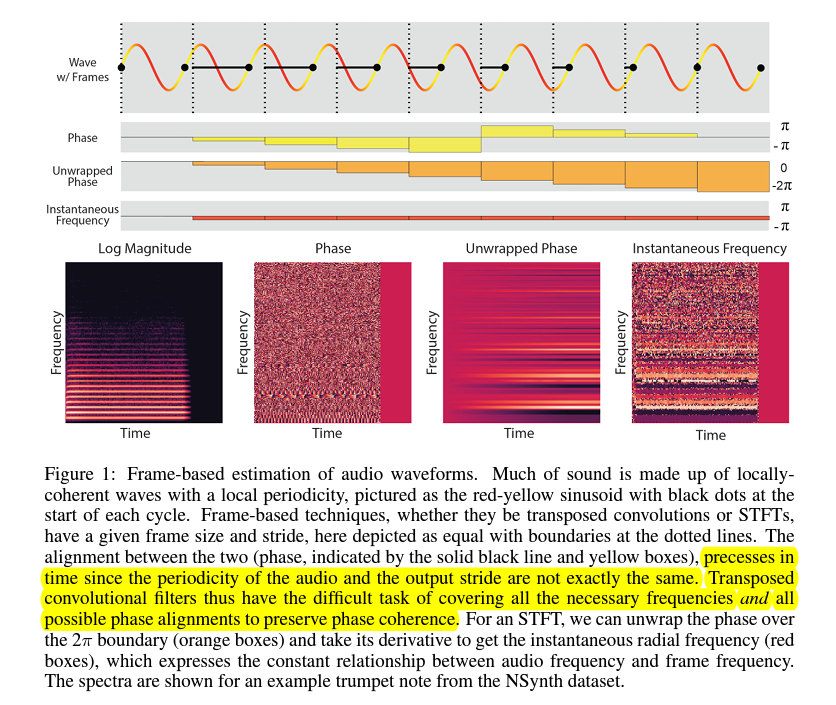
\includegraphics{fig_01.PNG} - Human perception highly sensitive to
doscontinuities and irregularities in periodic waveforms - Challenge for
synthesis network - It must learn all the correct frequency+phase
combinations to output a coherent waveform.

    This paper - 1. Generate log-magnitude spectrograms and phases directly
with GAN 2. \textbf{Estimate Instantaneuos Frequency Spectra(Rather than
Phase), more coherent audio}

    Dataset - - Nsynth(available online) - restricted to training on subsets
of accoustic instruemtns, and limited pitch range(MIDI 24-84
\textasciitilde{} 1000Hz)

    Architecture - - Progressive training of GAN's(Karras 2018a paper) -
Condition on additional source of information(pitch) to achieve
independent control of pitch and timbre

    Evaluation - 1. Human Evaluation 2. Number of Statistically Different
Bins(NDB) - measure diversity of generated samples 3. Inception Score 4.
Pitch accuracy, pitch entropy 5. Frechet Inception Distance

    Discussion - - Phase Coherence of generated waveforms(Rainbowgrams!)
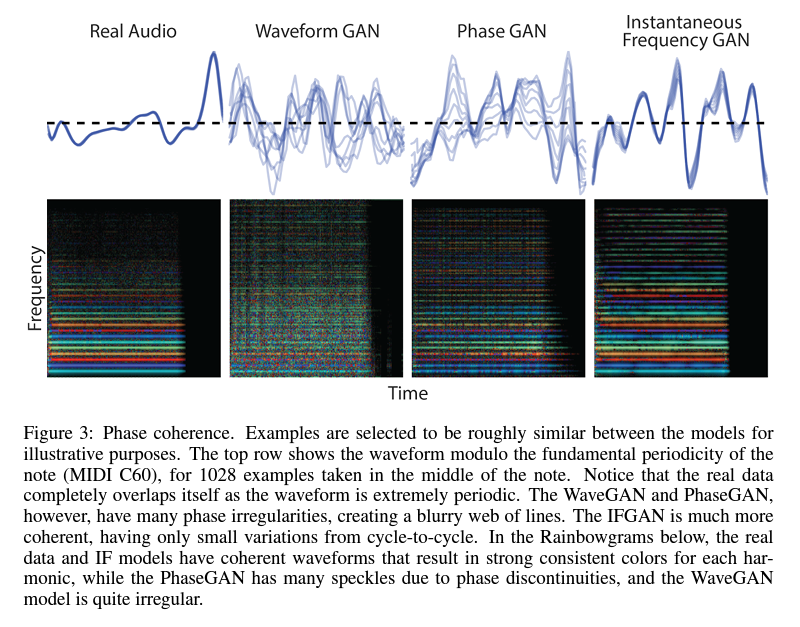
\includegraphics{fig_02.PNG} - Interpolation(\textbf{spherical
interpolation} vs linear interpolation in previous work) observed smooth
perceptual changes, no major artifacts - Consistent Timbre across pitch,
fix latent vector and condition on pitch. Timbral identity is constant
for given point in latent space. - Extremely fast generation

    Future Work - - Combining adversarial losses with encoders(use VAE to
model G and D) - More straightforward \textbf{regression losses} to
capture full data distribution

    \begin{center}\rule{0.5\linewidth}{\linethickness}\end{center}

\subsubsection{TIMBRETRON: AWAVENET(CYCLEGAN(CQT(AUDIO))) PIPELINE FOR
MUSICAL TIMBRE
TRANSFER}\label{timbretron-awavenetcyclegancqtaudio-pipeline-for-musical-timbre-transfer}

\href{http://www.cs.toronto.edu/~huang/TimbreTron/index.html}{Video} ***

    \begin{itemize}
\tightlist
\item
  Aim to solve problem of \textbf{Musical TImbre Transfer} i.e.
  manipulate timbre from one instrument to match another while
  preserving other musical content(pitch, rhythym, loudness)
\item
  Inspired by \textbf{Image Domain} style transfer techniques
\end{itemize}

    \begin{enumerate}
\def\labelenumi{\arabic{enumi}.}
\tightlist
\item
  Use the Constant-Q Transform(CQT) to obtain the TF representation of
  the audio(log magniutde, no phase)
\item
  CycleGAN for timbre transfer
\item
  Conditional Wavenet Synthesizer
\end{enumerate}

\begin{figure}
\centering
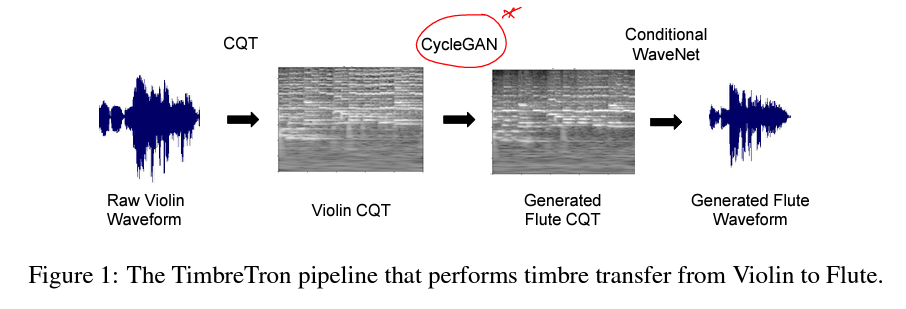
\includegraphics{fig_03.PNG}
\caption{process}
\end{figure}

    Why CQT? 1. Well suited for timbre due to pitch equivariance 2.
Simultaneuosly achieves better frequency resolution at low frequencies
and high temporal resolution at higher frequencies 3. Empirical
experiments yielded better performance compared to STFT 4. Outperformed
traditional representations like MFCC's in environmental sound
classifications using CNN's(Husaifah 2017)

Issues I felt 1. No phase 2. Not perfectly invertible(though they claim
it is)

    Dataset - Unrelated collections of different musical instruments(from
YouTube, links available in appendix)

    Architecture - 1. TF representation using log magnitude of CQT. 2.
\textbf{CycleGAN} - - Unsupervised domain transfer - learn a mapping
between two domains \textbf{without any paired data} 3. Reconstruction
from TF representation generated - - Avoid Griffin Lim as no optimality
guarantees - Hence, use conditional wavenet to generate waveform 4.
Major Contributions - 1. \textbf{Beam Search} - Possibility of producing
low-probability outputs sometimes. To avoid this, search through
Wavenet's generations to search output which better matches target CQT
2. \textbf{Reverse Generation} - Percussive attacks not modelled
correctly at onsets(difficult to determin onset from CQT). Solve by
generating samples backwards i.e. in reverse order(Really Cool Hack!!)
5. Also proposed architectural modifications for the following - 1.
Removing CHeckerboard artifacts 2. Full Spectrogram Discriminator 3.
Gradient Penalty 4. Identity Loss

    Discussion - - Evaluation primarily through human evaluation(Amazon
Mechanical Turk + feedback form) - Performed an \textbf{ablation} study
to analyze importance of different architectural changes + importance of
certain features - CQT well suited to convolutional architectures mainly
due to \textbf{pitch
equivariance}(\href{https://www.quora.com/What-is-the-difference-between-equivariance-and-invariance-in-Convolution-neural-networks}{What
this means in CNN's})

    \begin{center}\rule{0.5\linewidth}{\linethickness}\end{center}

\subsubsection{WAVENET: A GENERATIVE MODEL FOR RAW
AUDIO}\label{wavenet-a-generative-model-for-raw-audio}

\href{https://deepmind.com/blog/wavenet-generative-model-raw-audio/}{Audio
Examples} ***

    \begin{itemize}
\tightlist
\item
  Deep neural network to generate \textbf{raw audio waveform}(all the
  above methods generated TF representations which were inverted to
  obtain waveforms)
\item
  Fully \textbf{probabilistic + Autoregressive}
\item
  Inspired Heavily from previous work by same author i.e. PixelCNN to
  generate images pixel by pixel.
\end{itemize}

    \begin{itemize}
\tightlist
\item
  Models joint probability in the following way -
  \(p(\bar(x)) = \Pi_{t=1}^{T}(x_{t}|x_{1},\dots,x_{t-1})\) i.e. each
  sample depends on all the samples before it.
\item
  Use \textbf{Dilated Causal Convolutions} to model the above -
  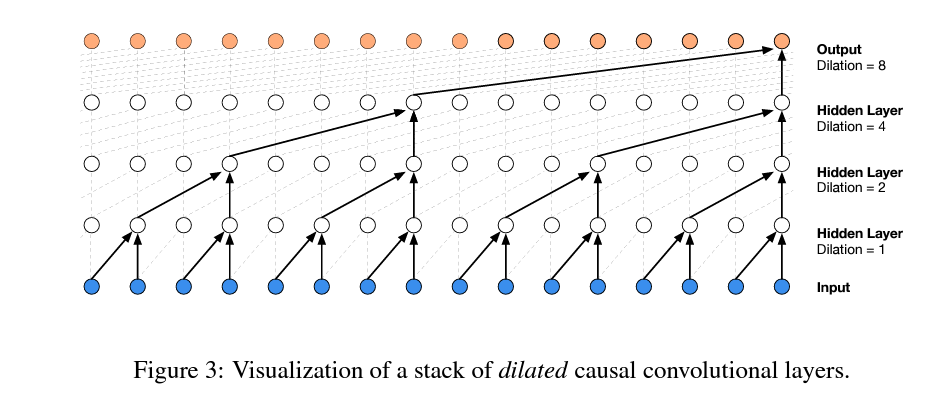
\includegraphics{fig_04.PNG}
\item
  \textbf{Softmax} vs \textbf{GMM} to model conditional distributions
\item
  \textbf{Gated Activation Units} works as a better non-linearity for
  audio signals vs ReLU
\item
  \textbf{Context Stacks} to increase Receptive Field size
\end{itemize}

    \textbf{Conditional Wavenets} - - Model conditional distribution given
an input h i.e.
\(p(\bar(x)|h) = \Pi_{t=1}^{T}(x_{t}|x_{1},\dots,x_{t-1},h)\). This is
done to produce audio with required characteristics(timbre, pitch) -
Done in two ways - 1. Global conditioning - Influence output at all time
steps 2. local conditioning

    Discussion - - Lack of long range coherence dut to limited size of
Receptive Field - Picks up certain other characteristics in audio such
as mimicking accoustics and recording quality(and breathing and mouth
movement for speakers in case of speech generation) - Large RF necessary
for Music! - Evaluation using \textbf{Mean Opinion Scores(MOS)} tests on
human evaluated samples.

    \begin{center}\rule{0.5\linewidth}{\linethickness}\end{center}

\subsubsection{Neural Audio Synthesis of Musical Notes with WaveNet
Autoencoders}\label{neural-audio-synthesis-of-musical-notes-with-wavenet-autoencoders}

\href{https://magenta.tensorflow.org/nsynth}{Website} ***

    \begin{itemize}
\tightlist
\item
  Inspired by Wavenet, they deisgn a Wavenet Style autoencoder, that
  conditions the decoder on \textbf{temporal codes} learnt from the raw
  audio waveform. These capture long term structure without external
  conditioning.
\item
  The model learns a \textbf{manifold of embeddings} that allows
  morphing, interpolations etc.
\end{itemize}

    Architecture 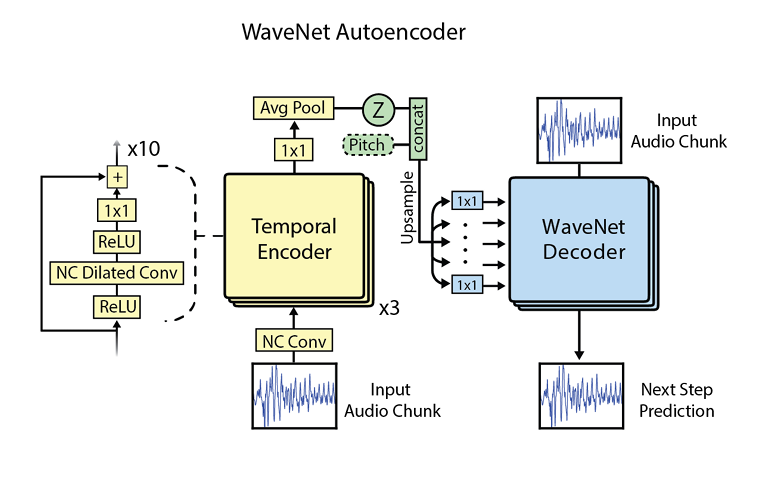
\includegraphics{fig_05.PNG}

Thus, instead of external conditioning, the input embeddings work as the
conditioning variable, which encodes information about the waveform
\(p(\bar(x)) = \Pi_{t=1}^{T}(x_{t}|x_{1},\dots,x_{t-1},f(\bar(x)))\)

Major Limitation - - Unable to fully capture global context due to
memory constraint(open problem)


    % Add a bibliography block to the postdoc
    
    
    
    \end{document}
